\documentclass{article}
\usepackage[margin=2cm, includefoot, footskip=30pt]{geometry}
\setlength\parindent{0pt}
\setlength{\parskip}{1em}
\usepackage{authblk}
\usepackage{pdfpages}

\title{Using a theory of mind to find best responses to memory-one strategies.}

\author{Nikoleta E. Glynatsi, Vincent A. Knight}

\begin{document}

\maketitle

We would like to open this response by thanking the reviewers for their
thoughtful comments and suggestions. We have fully taken their comments on board
and made significant modifications and additions to the manuscript.
We feel this has greatly improved the work. Given the nature of these changes,
we hope that the editorial team are willing to overlook the fact that
they stipulated that if any further modification are required the manuscript
would be rejected. Hopefully if further minor modifications are needed we will
be given the opportunity to make them.

Both reviewers commented on different aspects of the paper and so our
modifications naturally fit in to two categories (which we will discuss in
detail comment by comment):

\begin{itemize}
    \item The first reviewer suggested that the manuscript lacked discussion of
    noise and of the literature on the theory of mind. We address
    this including noise in our formulation (in the appendix) and by discussing
    relevant literature on the theory of mind (in the introduction).
    \item The second reviewer questioned the claims on the evolutionary
    stability of the best response and expressed that the manuscript would
    benefit from such experiments and discussion. To address this, we have
    have obtained expressions for the fixation probability of a best response
    strategy in a Moran process that adapts dynamically to the population.
\end{itemize}

We will now take each comment of the reviewers in turn and highlight our efforts
to improve the work.

\section{Response}

\textbf{Regarding the comments of Reviewer 1:}

\begin{verbatim}
    `` Noise or error (in implementing a move, e.g. due to trembling hand or
    fuzzy mind) is a crucial aspect in the context of the IPD. Given that noise
    is unavoidable in real-world applications of the IPD, it’s therefore important
    to take them into account. A relevant question is whether similar observations
    will be seen in noisy IPD? Authors should consider or at least discuss this
    important issues of IPD.''
\end{verbatim}

We agree with the reviewer that noise is an important aspect of research. Noise
is now included in the discussion, specifically pointing at the appendix where
we have obtained expressions for the utilities with noise.

\begin{verbatim}
    ``The paper lacks sufficient discussion of previous works, especially regarding
    the literature of theory-of-mind and complex strategies in repeated games.
    Authors should consider discussing this highly literature to improve the
    relevance of the paper.''
\end{verbatim}

We have discussed several articles
that have been proposed by the reviewer.

\textbf{Regarding the comments of Reviewer 2:}

\begin{verbatim}
    ``The structure despite having been improved quite a bit, still leaves something
    to be desired. For example, the contents of Section 1.2 were not fully moved
    into the appendix, but instead partially pop up in the discussion section.
    This interrupts the flow of the paper, as the discussion section is not the
    place for a new lemma. It would be better to make a reference to this result
    as a corollary to Theorem 1, and leave all details and Figure 4 to the appendix.''
\end{verbatim}

We have made changes in order to improved the narrative. This includes moving
Section 1.2 to the appendix, changing the order of our results and removing
the discussion of tournaments with self interactions.

\begin{verbatim}
    On that note, the lack of evolutionary results is somewhat disappointing,
    and the current results give no intuition if such a best response strategy,
    as described in the text, would arise in the evolutionary trajectory.
    The original manuscript was somewhat misleading in this regard, and even the
    revised version is a bit confusing, by mixing best response *dynamics*, best
    response strategies, and vague hints to learning/stochastic processes such
    as the Moran process into the results section without actually presenting
    results on this issue. Self-interactions do not equal an evolutionary setting,
    and best response does not automatically equal evolutionary stability.
    It would be crucial to clear up any confusion there, starting with
    further purging misleading references to any "evolutionary setting" from
    the text (e.g. the authors missed this in the caption for Fig.2).
\end{verbatim}

This particular comment proved fruitful for us as it lead to many
discussions and some interesting new work. Thank to the reviewer.

We note that we have not addressed whether or not a best response strategy would
arise in the evolutionary trajectory. This is because the best response strategy
is obtained using the quadratic ratio, essentially transforming the
problem to a finite dimensional optimisation problem. As such, an evolutionary
algorithm could be used to find the best response. However, in our particular case
Bayesian optimisation is the tool chosen. This does not offer insight as to
whether or not the best response strategy is on the evolutionary trajectory.
We have added a comment about this in the conclusion as it would prove to be an
interesting avenue for future work.

We have addressed the latter parts of this comment with a significant addition
of work to the manuscript. We no longer refer vaguely to Moran processes but
instead explicitly consider a Moran process where the best response player is
able to dynamically adapt to the population distribution (and a classic Moran
process). As well as the theoretic expressions obtained (modifications of the
standard results on Moran processes) this is coupled with a data set of
experiments on the Moran process. We feel that this is a strong addition to the
manuscript that ensures there is no further confusion.

\section{Marked changes made to the manuscript}

We are also attaching a copy of the revised manuscript where we have highlighted
the changes made to the originally submitted manuscript.

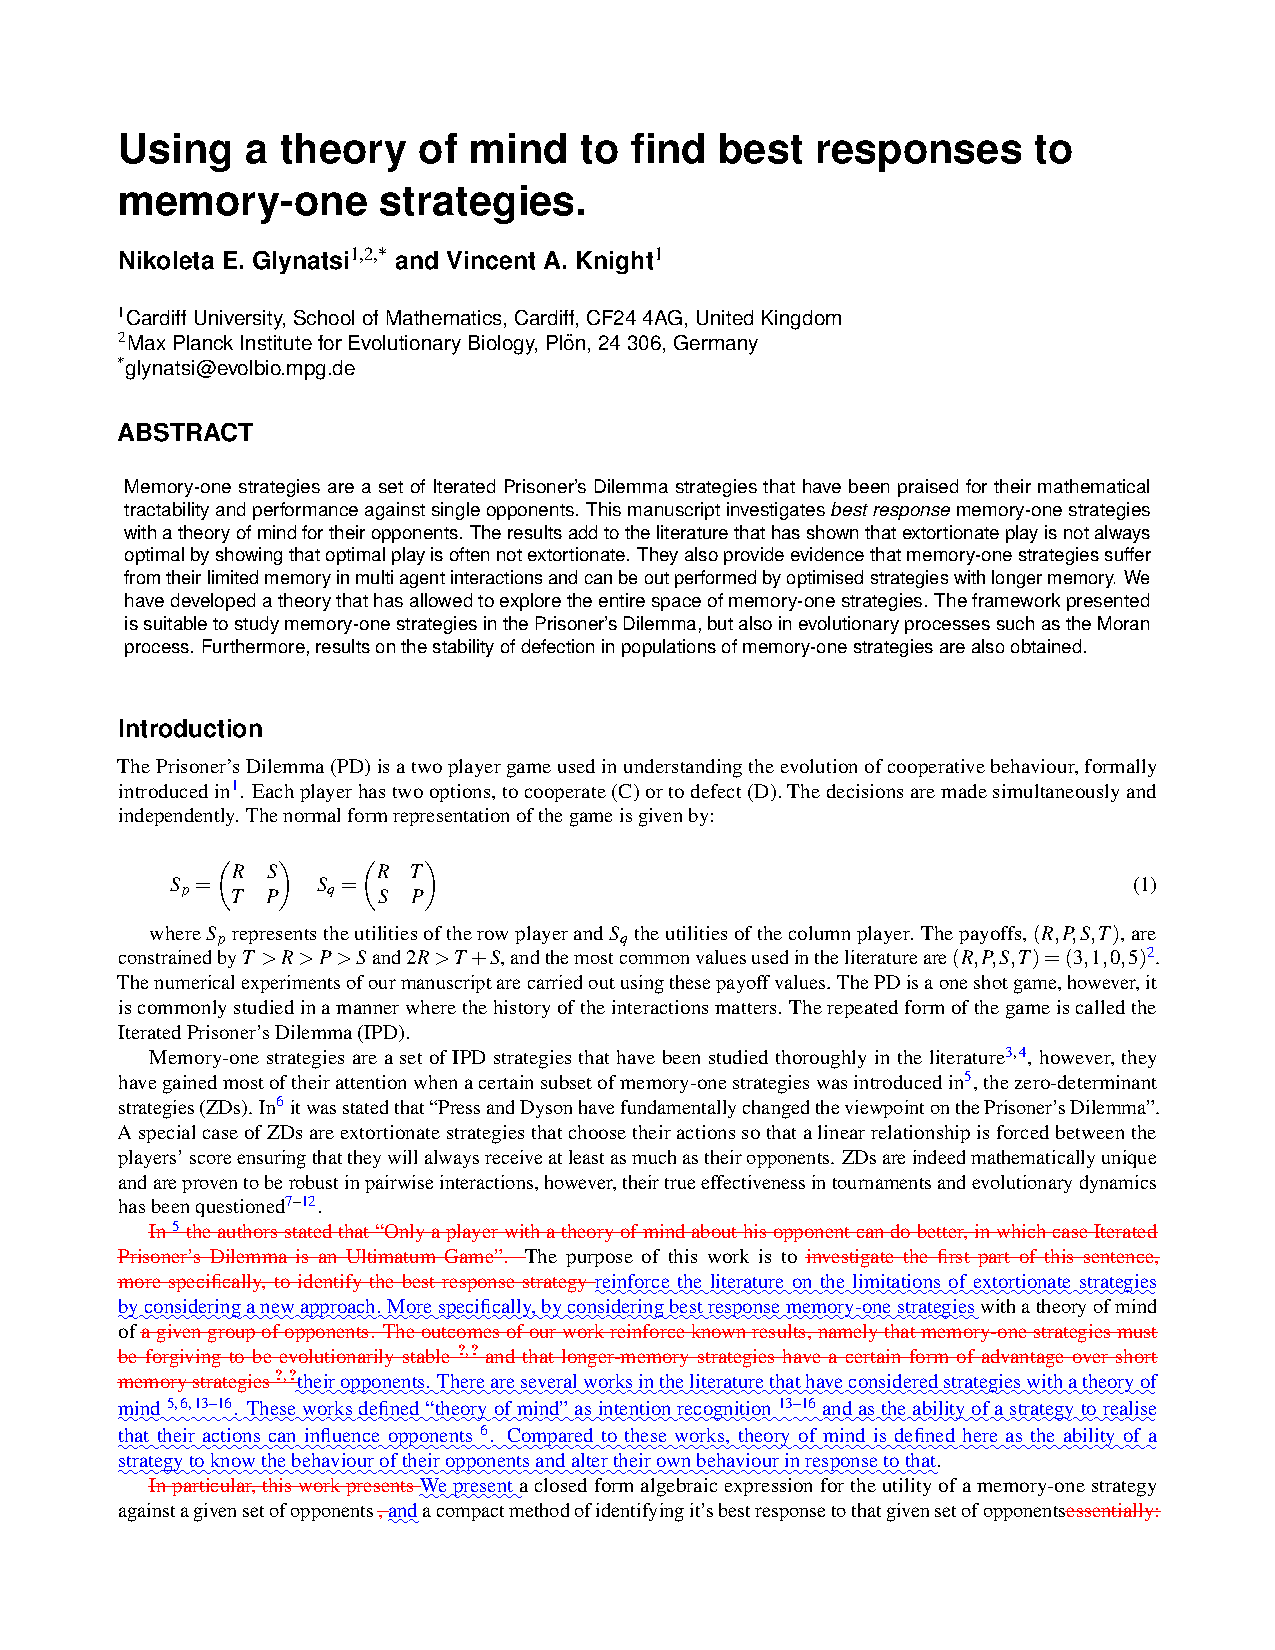
\includepdf[pages=-]{../diff.pdf}

\end{document}
